\chapter{Architecture}
\label{chap:arch}

The proposed system consists of several separately running subsystems. Breaking up functionality into discrete processes facilitates the integration of external applications to expand upon this work. For example, a user might want to use the system to create a semantic map but implement his own perception module in order to recognize different kinds of objects or to utilize other kinds of sensors. \\

Since most of the subsystems depend on information from other subsystems, they need a way to communicate with each other. To this end they specify interfaces that determine which information they provide and which information they need. These interfaces are defined in such a way that each subsystem stands at a certain stage of the data flow where all previous stages are (explicitly or implicitly) mandatory for the subsystem to run while all succeeding stages are optional. The visualization for instance marks the last stage and therefore requires information from all other stages to run: It depends explicitly on the database and the semantic map (because it displays information from those stages) and implicitly on the perception (because the semantic map depends explicitly on the perception).

\tikzstyle{build}=[
  rectangle,
  rounded corners,
  draw=black,
  very thick,
  text centered,
  text width=8cm,
  minimum height=12mm,
  fill=black!15,
  font=\sffamily
]

\tikzstyle{build2}=[
  rectangle,
  rounded corners,
  draw=black,
  very thick,
  text centered,
  text width=7.7cm,
  minimum height=12mm,
  fill=black!12,
  font=\sffamily
]

\tikzstyle{build3}=[
  rectangle,
  rounded corners,
  draw=black,
  very thick,
  text centered,
  text width=7.4cm,
  minimum height=12mm,
  fill=black!9,
  font=\sffamily
]

\tikzstyle{build4}=[
  rectangle,
  rounded corners,
  draw=black,
  very thick,
  text centered,
  text width=7.1cm,
  minimum height=12mm,
  fill=black!6,
  font=\sffamily
]

\begin{figure}[H]
  \centering
  \begin{tikzpicture}
    \node [build] (Vis) {
      \qquad \\
      4 - Visualisation \\[0.5\baselineskip]
      \begin{tikzpicture}
        \node [build2] (Map) {
          \qquad \\
          3 - Semantic Map \\[0.5\baselineskip]
          \begin{tikzpicture}
            \node [build3] (Rec) {
              \qquad \\
              2 - Perception \\[0.5\baselineskip]
              \begin{tikzpicture}
                \node [build4] (DB) {
                  1 - Database
                };
              \end{tikzpicture}
            };
          \end{tikzpicture}
        };
      \end{tikzpicture}
    };
  \end{tikzpicture}
  \caption{Startup order of subsystems: The contained subsystems need to run in order to start the containing subsystem.}
\end{figure}

\section{Datatypes}
\label{sec:arch-types}
Each object has two kinds of values: (1) Those that are the same for all objects of the same type and (2) those that are different for each instance. For example, all packs of cornflakes of one brand look the same and have the same dimensions, but they all have a different position. Analog to naming conventions in programming languages the first kind will be called \texttt{class attributes} and second \texttt{object attributes} in this document. \\

While object oriented programming languages already differentiate between class and object attributes by design, there are good reasons to break them up in the proposed system: A clear seperation allows each subsystem to handle one specific task without having to work around other aspects of this work.

For example, the semantic map might need an objects dimensions for some calculations, but it should not have to manage them, because they are not part of an object pose. In order to keep class and object attributes together, the class attributes would either have to be static or the semantic map would have to propagate updates to the dimensions through all memorised instances. Static attributes would rule out some functionality though, like remembering multiple candidates for the dimensions of an object in order to compute an average.

From a user perspective, the separation allows to decide which information can be found in which part of the system more intuitively. Someone who is interested in the dimensions of an object will assume them to be found in the database, rather than the semantic map. \\

\begin{table}[H]
  \centering
  \caption[The class attributes of an object.]{The class attributes of an object. These attributes hold true for all objects of the same type.}
  \label{tab:class-attributes}
  \renewcommand{\arraystretch}{1.5}
  \begin{tabularx}{\textwidth}{R{0.5} L{1.5}}
    \hline
    \multicolumn{2}{c}{\textbf{Class attributes}} \\
    \hline
    Type name     & The kind of object. Used not only to tell different types of objects apart, but also to identify the associated object attributes. \\
    Texture image & A photo of the object. This image will be compared with the robots camera image in order to detect the associated type of object in the world. \\
    Dimensions    & The width and height of an object in the real world. In combination with an objects position the width and height tell a robot where the object starts and ends, which is essential for the object to be grasped correctly. \\
    Confidence    & Measurement for the reliabilty of the dimensions. If an object is recognized multiple times, the quality of the width and height values can be improved by weighting more reliable data higher. \\
    \hline
  \end{tabularx}
\end{table}

\begin{table}[H]
  \centering
  \caption[The instance attributes of an object.]{The instance attributes of an object. These attributes are different for each instance of an object.}
  \label{tab:object-attributes}
  \renewcommand{\arraystretch}{1.5}
  \begin{tabularx}{\textwidth}{R{0.5} L{1.5}}
    \hline
    \multicolumn{2}{c}{\textbf{Object attributes}} \\
    \hline
    Type name            & The kind of object. Used to identify the associated class attributes. \\
    Unique ID            & Instances need a unique ID in addition to their type in order to tell them apart. \\
    Coordinate system ID & The coordinate system in which the objects position and orientation are specified. Objects are detected from the camera point of view but need to be placed in a static world coordinate system, because the camera moves. \\
    Position             & The position of the object. \\
    Orientation          & The orientation of the object. \\
    Confidence           & Measurement for the reliabilty of the 3D pose. If an object is recognized multiple times, the quality of the position and orientation can be improved by weighting more reliable data higher. \\
    \hline
  \end{tabularx}
\end{table}

\section{Database}
\label{sec:arch-db}
The database is the starting point for the system. The objects it is supposed to look out for are defined here, i.e. their name and the image required to detect them. Additionally the database holds the other class attributes (see table~\ref{tab:class-attributes}), i.e. the width and height of an object, and updates them according to the perceived dimensions. \\

Several interfaces enable other subsystems to add new types of objects to the database. Since the dimensions will be calculated by the perception, only a name and an image of the object are required upon initialization. The image can be provided directly through the interface, but the database is able load images from the harddrive, thus a path to a file is sufficient.

Whenever a new object is added to it, the database will broadcast a notification to the other subsystems, informing them about the addition. A subsystem using information from the database then would request the new list of objects if necessary and process it accordingly. \\

\begin{table}[H]
  \centering
  \caption[Database add-images interface]{Images can be provided through this interface to add new objects to the database.}
  \label{tab:db-add-images}
  \renewcommand{\arraystretch}{1.5}
  \begin{tabularx}{\textwidth}{R{0.5} L{1.5}}
    \hline
    \multicolumn{2}{c}{\textbf{Add image(s)}} \\
    \hline
    Image[]     & A list of sample images to be added to the database. Each image defines a new object. \\
    Type name[] & A list of names associated with the sample images. These names will be used to identify the objects. \\
    \hline
  \end{tabularx}
\end{table}

\begin{table}[H]
  \centering
  \caption[Database add-files interface]{Paths to image files can be provided through this interface to add new objects to the database.}
  \label{tab:db-add-files}
  \renewcommand{\arraystretch}{1.5}
  \begin{tabularx}{\textwidth}{R{0.5} L{1.5}}
    \hline
    \multicolumn{2}{c}{\textbf{Add file(s)}} \\
    \hline
    Path[]                 & A list of paths pointing to sample images on the harddrive, to be loaded and added to the database. Paths can point to single files or directories containing multiple images. Each image defines a new object. \\
    Type name[] (optional) & A list of names associated with the sample images. These names will be used to identify the objects. If no names are provided, the filenames (sans extension) will be used as typenames. \\
    \hline
  \end{tabularx}
\end{table}

The content of the database can be accessed via an interace which just returns all objects currently existing. If a subsystem knows the typename of the object it wants to access, there is another service which only returns the corresponding object. \\

\begin{table}[H]
  \centering
  \caption[Database getter interfaces]{Interfaces to access the contents of the database.}
  \label{tab:db-get-all}
  \renewcommand{\arraystretch}{1.5}
  \begin{subtable}[t]{.495\linewidth}
    \vspace{0pt}
    \begin{tabularx}{\textwidth}{R{0.75} L{1.25}}
      \hline
      \multicolumn{2}{c}{\textbf{Get all objects}} \\
      \hline
      Class attributes[] (Output) & A list of all objects currently defined in the database. \\
      \hline
    \end{tabularx}
  \end{subtable}%
  \rowcolors{1}{black!6}{white}
  \hfill
  \begin{subtable}[t]{.495\linewidth}
    \vspace{0pt}
    \begin{tabularx}{\textwidth}{R{0.75} L{1.25}}
      \hline
      \multicolumn{2}{c}{\textbf{Get object by type}} \\
      \hline
      Type name (Input) & The name of the object that is to be accessed. \\
      Class attributes (Output) & The class attributes of the object associated with the given type name. \\
      \hline
    \end{tabularx}
  \end{subtable}%
\end{table}

Since the database handles them too, it listens to what dimensions the perception calculates for successfully recognized objects. It uses this data to approximate an objects real dimensions, by computing an average over multiple occurences of the object and weighting them with their corresponding confidence. Note that it is not mandatory to make use of this interface. The database does manage dimensions when provided, but simply ignores them otherwise.

\section{Perception} % Dedicated subsection about OpenNI / RGB-D camera?
\label{sec:arch-perception}
The perception is responsible for processing camera images to detect objects and calculate their position. It requires a camera that provides color or grayscale images as well as depth images. \\

Color or grayscale images are needed for the object detection. The perception compares each camera image to the image of each object in the database. If the image of an object occurs as part of the camera image, the depth image is required to calculate the 3D position of the occurence. To this end it is essential, that the image streams of the camera and depth images are synchronized, i.e. both images are provided for the same moment in time. Synchronization ensures that the information from the depth image can be attributed to the corresponding position in the camera image. \\

Images from objects in the database need to be pre-processed in order to detect them in a camera image. Since images in the database rarely change, the perception can fetch all of them at once, process them and store the processed state (instead of processing them before every attempt to match them to the camera image). This means of course, that it needs to listen for changes to the database, because it needs to retrieve and process newly added objects. \\

In order to communicate information about recognized objects to other subsystems, the perception provides three interfaces: It broadcasts (1) the objects dimensions, (2) the objects position and orientation and (3) the camera position and orientation from where the object was seen.

The information is broadcast seperately, so that it can be processed by different subsystems without unnecessary overhead. In this work, (1) is handled by the database and (3) is handled by the semantic map. Note that (2) is not used in this work at all, but is already existing information that may be used in future work.

The information is broadcast simultaneously though, because a user might want to implement different or additional subsystems that need to associate the various parts with each other.

\section{Semantic Map}
\label{sec:arch-map}
The semantic map handles objects recognized by the perception. This includes memorising the various instances of objects the robot comes across during his work, checking if memorized objects are still there, updating objects that changed since they were last seen and resolving conflicts that occur when multiple objects are detected at the same position. \\

The semantic map receives to the object poses broadcast by the perception and compares them to the objects it already accumulated. If it already memorized an object of the same type at the same position, it assumes that it is dealing with the same object. In this case the previously calculated object pose can improved by computing the average of the existing and the new pose, weighted by how confident the perception was about these values.

In order to check if two objects overlap, the semantic map needs to retrieve the dimensions associated with the type of object from the database. \\

When other processes need an object, they can query the semantic map for where it is most likely to be found within a preferably close range. This means that the semantic map needs to be able to evalute objects by their distance to the current camera position and by how much time has passed since the object was detected.

Objects memorized by the semantic map can be accessed via multiple interfaces that filter objects by the following categories: (1) All currently stored objects, (2) all objects of a specific type, (3) all objects within a given range around a specific position and (4) all objects inside the cameras current field of view.

Note that all interfaces provide a set of all viable alternatives for a request rather than a single best candidate. The sets are sorted according to an evaluation function as a suggestion to the enquirer, enabling him to move on to the next best option as needed.

\section{Visualization}
\label{sec:arch-viz}
The visualization takes on the roll of a user who wants to work with the new information provided by the proposed system. It serves as an example on how to use the application, as well as providing a visual presentation of the internal state of the semantic map and related information from the database.

\begin{figure}[H]
  \centering
  \begin{tikzpicture}[
    ->,
    auto,
    swap,
    vertex/.style={
      rectangle,
      rounded corners,
      fill=black!12.5,
      draw=black,
      very thick,
      text centered,
      text width=3cm,
      minimum height=9mm,
      font=\sffamily
    },
    edge/.style={
      draw,
      very thick,
      line width=1.5pt,
      inner sep=3pt,
      outer sep=3pt,
      font=\sffamily,
    }
  ]
    % Nodes.
    \node [vertex] (e) {RGB-D Camera};
    \node [] (e_img) [above left = -1cm and -1.7cm of e] {
      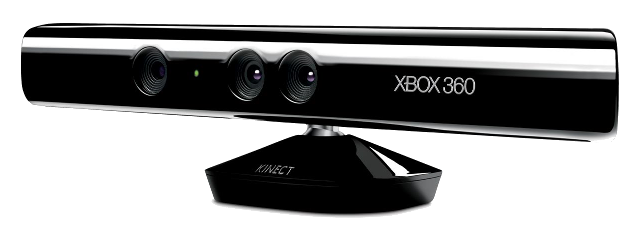
\includegraphics[width=128pt]{images/kinect.png}
    };
    
    \node [vertex] (b) [below       = 2cm         of e] {Perception};
    
    \node [vertex] (a) [below left  = 2cm and 3.5cm of b] {Database};
    \node [] (a_img) [above = 3.5cm of a] {
      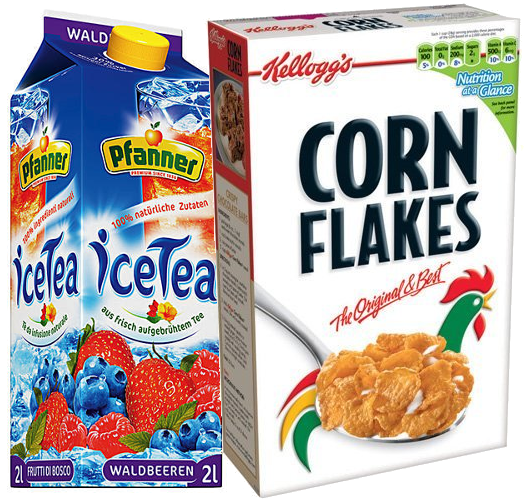
\includegraphics[width=96pt]{images/objects.png}
    };
    
    \node [vertex] (c) [below = 2cm of b] {Semantic Map};
    \node [vertex] (d) [below = 2cm of c] {Visualization};
    % Database <-> Perception.
    \path [edge] (a) edge [bend left] node [left, align=center] {object names, \\ sample images} (b);
    \path [edge] (b) edge [] node [right, align=center] {object \\ dimensions} (a);
    % Perception -> Semantic Map.
    \path [edge] (b) edge [] node [right] {3D object poses} (c);
    % Database -> Semantic Map.
    \path [edge] (a) edge [] node [] {object dimensions} (c);
    % Database -> Visualization.
    \path [edge] (a) edge [] node [left, align=center] {object names \\ \& dimensions} (d);
    % Semantic Map -> Visualization.
    \path [edge] (c) edge [] node [right] {3D object poses} (d);
    % Kinect -> Perception
    \path [edge] (e) edge [] node [right, align=center] {camera images, \\ depth images} (b);
    % Objects -> Database
    \path [edge] (a_img) edge [bend right] node [] {} (a);
  \end{tikzpicture}
  \caption{Dataflow between the subsystem.}
\end{figure}
